\documentclass[11pt, a4paper]{article}
\usepackage[nochapters]{classicthesis}                              % template
\usepackage[margin=42mm]{geometry}                                  % margins
\usepackage[utf8]{inputenc}                                         % allow utf-8 input
\usepackage[T1]{fontenc}                                            % use 8-bit T1 fonts
\usepackage{graphicx}                                               % images
\usepackage{url}                                                    % URL typesetting
\usepackage{booktabs}                                               % good-looking tables
\usepackage{multirow}                                               % for tables
\usepackage{amsfonts}                                               % blackboard math symbols
\usepackage{amsmath}                                                % math ops
\usepackage{nicefrac}                                               % compact 1/2, etc.
\usepackage{microtype}                                              % microtypography

\definecolor{darkblue}{rgb}{0, 0, 0.5}                              % define link color
\hypersetup{colorlinks=true,citecolor=darkblue,                     % set link color
            linkcolor=darkblue, urlcolor=darkblue}

% Your packages here
% \usepackage{...}                                                  % some info, maybe

% !!! PLEASE CHANGE THESE VARIABLES TO MATCH YOUR INFORMATION !!!

\def\thesistitle{Multi-class Alzheimer's Disease classification from structural MRI using Vision Transformers}                      % title
\def\subtitle{A comparison of data-efficient and hierarchical Vision Transformers}             % subtitle
    % ^if there is no subtitle, replace by \def\subtitle{}  
\def\yourname{M.D.W. van der Wielen}                                                                       % ^first and last name
\def\yourprogramme{Data Science \& Society}                         % OR (remove this)
% \def\yourprogramme{Cognitive Science \& Artificial Intelligence}    % uncomment this
\def\yourstudentnumber{2027613}                                      % ANR (or u-number)
\def\finalmonth{January}
\def\finalyear{2000}
\def\supervisor{dr. J. S. Olier Jauregui}
\def\committee{dr. G. Saygili}
\def\acknowledgments{Some room for acknowledgements.}

% METADATA

\hypersetup{pdfauthor   = \yourname,
            pdftitle    = \thesistitle\ \subtitle,
            pdfsubject  = \yourprogramme\ Master Thesis
}

% CHOOSE EITHER OF -----------------------------------------
% IEEE STYLE:

% \usepackage[square,numbers]{natbib}                               % bracket-style refs
% \usepackage{natbib}                                               % OR: parenthesized refs
% \bibliographystyle{IEEEtranN}

% OR -------------------

\usepackage[natbibapa]{apacite}                                     % only parentheses
\bibliographystyle{apacite}                                         % 'cause APA

% !!! ------------------------------------------------------ !!!

\begin{document}
% DON'T TOUCH THIS FILE, THANKS!

\pagenumbering{gobble}
\thispagestyle{empty}

\newgeometry{margin=30mm}
\begin{center}
\hspace{0.75cm}
\includegraphics[scale=0.5]{logo.eps} \\
\vspace{5cm}
\huge\spacedallcaps{\thesistitle} \\ [0.5cm]
\Large\spacedallcaps{\subtitle} \\ [1.2cm]
\normalsize\spacedallcaps{\yourname{}} \\ [1cm]
\normalsize{\spacedlowsmallcaps{Thesis submitted in partial fulfillment}} \\
\normalsize{\spacedlowsmallcaps{of the requirements for the degree of}} \\
\normalsize{\spacedlowsmallcaps{Master of Science in \yourprogramme{}}}\\
\normalsize{\spacedlowsmallcaps{at the School of Humanities and Digital Sciences}} \\
\normalsize{\spacedlowsmallcaps{of Tilburg University}} \\ [5cm]
\normalsize{\spacedlowsmallcaps{Word count: ...}} \\
\end{center}
\restoregeometry

\newpage

\begin{tabular}{l}
\noindent \spacedlowsmallcaps{student number} \\ [0.2cm]
\yourstudentnumber \\ [0.5cm]
\spacedlowsmallcaps{Committee} \\ [0.2cm]
\supervisor \\
\committee\\ [0.5cm]
\spacedlowsmallcaps{location} \\ [0.2cm]
Tilburg University    \\                        
School of Humanities and Digital Sciences \\
Department of Cognitive Science \& \\
Artificial Intelligence \\
Tilburg, The Netherlands \\ [0.5cm]
\spacedlowsmallcaps{date} \\ [0.2cm]
\today \\
\end{tabular}
\vfill
\begin{tabular}{p{12cm}}
\spacedlowsmallcaps{acknowledgments} \\ [0.2cm]
%\noindent \acknowledgments{}
Firstly, I want to thank J. S. Olier Jauregui for his useful feedback and insights throughout the writing of this thesis. His guidance helped me write a thesis that aligned with the goals that I set at the start of the period. Secondly, I want to thank G. Saygili and E. Postma for the useful discussions and feedback that ultimately shaped my thesis. Finally, I want to thank my family, friends and girlfriend for supporting me during this period.
\end{tabular}

\newpage \pagenumbering{arabic}

\title{\rmfamily\normalfont\spacedallcaps{\thesistitle}\\[0.2cm]
       \rmfamily\small\spacedallcaps{\subtitle}}
\author{\spacedlowsmallcaps{\yourname}}
\date{}

\maketitle  % don't remove this :)

% --- start writing below:

\begin{abstract}
The currently ongoing negative trends concerning Alzheimer’s Disease (AD) call for improved methods for early AD detection. Mild Cognitive Impairment (MCI) is the prodromal stage of AD. Detecting MCI early could give room for opportunities to slow down or completely prevent the conversion to AD. For a long time, 2D and 3D convolutional neural networks (CNN) have been superior in classifying AD stages. The relatively new Vision Transformer (ViT) shows promising results in all computer vision domains. However, the need for large-scale datasets and high computational power limits their applicability to medical image classification. Therefore, the Data-efficient image Transformer (DeiT) and Swin Transformer are investigated in this research. The DeiT is better able to deal with small-scale datasets. The linear computational complexity of the hierarchical Swin Transformer makes it more computationally efficient compared to other ViTs. The ViT models are compared against VGG16, a state-of-the-art 2D CNN. The models are trained on a pre-processed AD dataset from the Kaggle website, after which they are evaluated on accuracy, precision, recall, the F1-score, and training time. The VGG16 beats the DeiT and Swin on accuracy by 4.2\% and 5.8\% respectively, achieving an accuracy of 91.9\%. An arguably more important metric for this research is the recall of the ‘mild demented’ class. For this class, the DeiT and Swin achieve a recall of 68.9\% and 66.7\% respectively. The VGG16 outperforms them with a substantially higher recall of 83.0\%. Therefore, it can be concluded that 2D CNNs remain the best-performing models for AD classification, and more research is necessary to unlock the full potential of ViTs.
\end{abstract}

\newpage

\section{Data source / code / ethics statement}
Work on this thesis did not involve collecting data from human participants or animals. The publicly available Alzheimer’s Disease dataset was obtained from the Kaggle website through \href{https://www.kaggle.com/datasets/tourist55/alzheimers-dataset-4-class-of-images}{\textbf{this}} link. The MRI images in the dataset are anonymized. The original owner of the data used in this thesis retains ownership of the data during and after the completion of this thesis. The author of this thesis acknowledges that they do not have any legal claim to this data. All figures and tables used in this thesis were produced by the author. The code used in this thesis is publicly available on GitHub here: \url{https://github.com/MathijsvdW/Master-Thesis}. 


\section{Introduction} \label{sec:introduction}
Alzheimer’s Disease (AD) is a progressive neurological disorder where the degeneration of nerve cells in the brain causes memory loss, decreased cognitive abilities, and personality change. It can eventually lead to death caused by complete brain failure \citep{BrightFocusFoundation2022Alzheimers:Stats}. Research has agreed upon the fact that brain changes occur due to an accumulation of abnormal proteins and phosphorylated tau in the brain \citep{AlzheimersAssociation20222022Figures}. A recent study indicates that AD progression may also be caused by a decrease in hard cognitive demand later in the lifespan \citep{Turknett2022DemandDementia}.

The importance of early AD detection and prevention becomes clear when looking at the trends in AD over the past decades. In 2010, there were 35.6 million people over the age of 60 worldwide that are living with the disease. This number is expected to almost double every 20 years, which means that by 2050 the amount of people living with AD is expected to be around 115 million \citep{Prince2013TheMetaanalysis}. In addition, deaths caused by dementia have increased by 139\% between 2000 and 2016 \cite{AlzheimersDiseaseInternational2020DementiaStatistics}. Together with other types of dementia, AD is expected to be the most expensive chronic disease in terms of nursing costs \citep{Ebrahimighahnavieh2020DeepReview}. The global cost of dementia per year was \$1.3 trillion in 2020, but 10 years later \cite{AlzheimersDiseaseInternational2020DementiaStatistics} is estimating that this amount will more than double to \$2.8 trillion by 2030.


According to a literature review by \cite{Ebrahimighahnavieh2020DeepReview}, 2D CNNs and 3D CNNs were competing as state-of-the-art Deep Learning models in detecting AD. However, a few very recent studies found that the relatively new Vision Transformer (ViT) also gives promising results \citep{Lyu2022ClassificationTransformer,Sarraf2022OViTAD:Data}. A milestone paper by \cite{Dosovitskiy2020AnScale} showed that the Transformer for Natural Language Processing (NLP) tasks also had great applications in computer vision tasks, by formulating image classification as a sequence prediction task of the image patch sequence \citep{He2022TransformersReview}. The ViT captures long-range dependencies with self-attention layers as introduced by \cite{Vaswani2017AttentionNeed}. This characteristic of ViT is ideal for brain imaging analysis, as MRIs are highly complex images where brain regions far away from each other may have strong relationships \citep{Lyu2022ClassificationTransformer}. A literature review on ViTs in the medical imaging domain by \cite{He2022TransformersReview} concluded that ViTs are slowly outperforming CNNs on most tasks. The only three studies that have tried to predict AD using ViTs are published in 2022, all with promising results \citep{Lyu2022ClassificationTransformer,Sarraf2022OViTAD:Data,Yin2022SMIL-DeiT:MultipleClassification}. To further investigate the performance of ViTs for AD classification the following research question is formulated: 

\begin{quote}
\centering
\emph{How do Vision Transformers perform in classifying multiple Alzheimer’s Disease stages?}
\end{quote}

\noindent ViTs are achieving high performance in several computer vision tasks such as object detection \citep{Fang2021YouDetection}, segmentation \citep{Ye2019Cross-modalSegmentation}, and classification \citep{Dosovitskiy2020AnScale}. However, a few challenges arise in the medical image classification domain. The challenges are mainly the computational cost and the lack of sufficient data for training the models \citep{He2022TransformersReview}. Clinical experts need to label the data, which is a time-consuming, error-prone, and expensive process \citep{Alzubaidi2021NovelData}. Therefore, two ViT models are chosen that are able to at least partially address the main challenges in AD classification using ViTs. This leads to the following sub-questions:

\begin{itemize}
\centering
    \item[SQ1] \emph{How does the data-efficient Vision Transformer compare to the baseline 2D CNN in classifying multiple AD stages?}
    \item[SQ2] \emph{How does the computationally-efficient Vision Transformer compare to the baseline 2D CNN in classifying multiple AD stages?}
\end{itemize}

\noindent To answer SQ1, a Data-efficient image Transformer (DeiT) is compared to a 2D CNN baseline model: VGG16. The DeiT is an improved ViT model, which achieves great performance on small-scale data due to improved training and a novel distillation procedure \citep{Touvron2021TrainingAttention}. The distillation procedure uses a  teacher-student strategy specific to transformers. The student learns from the teacher through attention using a distillation token.
The DeiT has a quadratic computational complexity with respect to image size, just like many other ViT models. The VGG16 model has proven to have great performance in AD classification tasks and was therefore chosen to function as the baseline model for this research \citep{Billones2017DemNet:Impairment,Hon2017TowardsLearning,Jain2019ConvolutionalImages}.

SQ2 is answered by comparing the performance of the Swin Transformer with VGG16. The Shifted Windows (Swin) Transformer by \cite{Liu2021SwinWindows} uses hierarchical feature maps. It divides an image into small patches and slides a local window over the image. It merges these image patches in deeper layers of the model. The self-attention is only computed in the non-overlapping local windows, but due to the merging patches in deeper layers it still allows for a cross-window connection. Unlike the DeiT and many other ViT models, the Swin Transformer has a linear computational complexity. Because of the computational efficiency, the Swin Transformer was chosen for this research. All the models are pre-trained on ImageNet-1k \citep{Deng2009ImageNet:Database}, which ensures that comparison of the models is unbiased. The models are evaluated on the following metrics: accuracy, precision, recall, the F1-score, and training time.

\newpage

\section{Related Work}
This section will start by reviewing the literature up until ViTs were introduced. After that, the ViTs are discussed and specifically examined with regard to the medical image analysis domain. The challenges in that domain will result in the model choices for this research. Finally, the chosen models are discussed.

\subsection{The rise of CNNs} \label{subs:CNN}
According to an extensive literature review by \cite{Ebrahimighahnavieh2020DeepReview}, research on deep learning for AD detection started in 2013. Since then, the amount of literature on the topic has increased substantially each year. The attempt to classify patients with MCI and AD through MRI scans started with Machine Learning approaches. However, \cite{Razzak2018DeepMaking} and \cite{Ebrahimighahnavieh2020DeepReview} concluded that traditional Machine Learning approaches do not compare to more recent Deep Learning models because of the high complexity of MRI imaging. \cite{Ebrahimighahnavieh2020DeepReview}, also show that about 90\% of the literature using Deep Learning to detect AD used a dataset from the Alzheimer’s Disease Neuroimaging Initiative (ADNI). ADNI is a longitudinal, multicentre study that performs extensive quality checks on their neuroimaging. The four main methods for extracting features from MRI are voxel-based, ROI-based, patch-based, and slice-based. The latter is used for this research because the other three methods require expert knowledge or high computational power due to 3D imaging. The slice-based method takes slices from one or more MRI planes. The planes are coronal (frontal), sagittal (median), and axial (horizontal). The dataset used in this research consists of slices from the axial plane. The breakthrough of CNNs after they won the ImageNet LSVRC-2010 competition was noticed by many researchers in the medical image analysis domain. \cite{Ebrahimighahnavieh2020DeepReview} show that 2D CNNs and 3D CNNs were the best-performing models in detecting AD for a long time. In most of the studies, the CNNs were trained from scratch, which resulted in inefficient model training. Transfer learning made it possible to transfer the training knowledge gained from one task to another. It is proven that transfer learning is faster and achieves better results, even with unrelated tasks \citep{Valliani2017DeepDiagnosis,Hon2017TowardsLearning}.
 A pre-trained 2D CNN that achieved great results in AD classification is VGG16. VGG16 is a 16-layer network built by Oxford's Visual Geometry Group (VGG) \citep{Simonyan2014VeryRecognition}. It won the ImageNet ILSVRC-2014 competition, mainly because it was one of the first networks that pushed to 16 layers with small convolution filters. \cite{Hon2017TowardsLearning} achieved a 74.1\% accuracy for two-way classification with a VGG model trained from scratch, and a substantial improvement to 92.3\% accuracy when using transfer learning. Similarly, \cite{Billones2017DemNet:Impairment} modified the VGG architecture by adding drop-out layers after each pooling layer and three fully connected layers. This architecture achieved a 91.9\% accuracy for the three-way classification of CN vs MCI vs AD. A more recent study by \cite{Jain2019ConvolutionalImages} also used the VGG16 that was trained on ImageNet for their three-way classification task. They only added classification layers and beat the state-of-the-art models with a 95.73\% accuracy. The increase in accuracy compared to the study from \cite{Billones2017DemNet:Impairment} might come from the MRI slice selection method. While both \cite{Jain2019ConvolutionalImages} and \cite{Hon2017TowardsLearning} used image entropy to select the most informative slices, \cite{Billones2017DemNet:Impairment} just took the middle 20 slices.

 \subsection{Vision Transformers} \label{subs:ViT}
The milestone paper by \cite{Vaswani2017AttentionNeed} revolutionized the Natural Language Processing (NLP) domain. It introduced an attention mechanism that would connect the encoder and decoder. The attention mechanism was initially intended for NLP tasks, becoming the de-facto standard in that domain. In the upcoming years, the attention mechanism would be used in conjunction with CNNs \citep{Wang2018Non-localNetworks,Carion2020End-to-EndTransformers}. However, the attention mechanism was also implemented in the computer vision field in the form of a ViT. The paper 'An image is worth 16x16 words' by \cite{Dosovitskiy2020AnScale} builds upon the research from \cite{Vaswani2017AttentionNeed} and used the attention mechanism for image classification, without using CNN-like architectures in their model. They showed that the ViT is able to perform great without the convolutional layers. The ViT takes an input image of size 224x224 and divides it into image patches of 16x16. These image patches are linearly embedded and are assigned a positional embedding so the transformer can keep track of the original image patch location. The 1D vectors of the image patches are multiplied by an embedding matrix, after which they are fed into the transformer encoder model along with their respective positional embeddings and an extra learnable class token. Within the transformer encoder is the multi-head self-attention mechanism implemented from \cite{Vaswani2017AttentionNeed}. A Multi-Layer Perceptron (MLP) head receives an output from the transformer encoder after which it performs the classification. 

\subsection{Vision Transformers in the medical image analysis domain} \label{subs:ViTmedical}
A study by \cite{Matsoukas2021IsImages}, investigated the performances of CNNs and ViTs. They performed experiments based on three mainstream medical image datasets and concluded that CNNs trained from scratch achieved better performance compared to ViTs trained from scratch. However, when pre-trained on ImageNet basic ViTs with default hyperparameters bridged the gap to CNNs. ViTs outperformed the CNN models when they were pre-trained using self-supervision. Similarly, a few very recent studies found that ViTs achieve comparable and occasionally better results than the state-of-the-art CNNs for AD classification \citep{Lyu2022ClassificationTransformer, Sarraf2022OViTAD:Data}. Even though CNNs can detect local features, they fail to capture long-range dependencies in distant brain regions \citep{He2022TransformersReview}. \cite{Lyu2022ClassificationTransformer} conclude that ViTs on the other hand are able to effectively capture these long-range dependencies. This is beneficial for brain image analysis because distant brain regions may have strong relationships with each other. This is in line with \cite{Gunawardena2017ApplyingData}, as they state that the advantage of the long-range dependencies in the AD detection domain is that the brain changes that indicate AD occur in distant parts of the brain, namely the hippocampus, cortex, and ventricle. 
The literature review on ViTs for medical image analysis by \cite{He2022TransformersReview} shows that ViTs are being used for CT scans, X-Ray, MRIs, histological images, and others. Out of those modalities, MRI was studied the least at the moment of review, with only four studies. Two of those involved brain MRI but neither of them focused on AD classification. Three other studies that did focus on AD classification using ViT are published in the last year, which shows that using ViTs for AD prediction is a relatively new approach \citep{Lyu2022ClassificationTransformer,Sarraf2022OViTAD:Data,Yin2022SMIL-DeiT:MultipleClassification}. \cite{Lyu2022ClassificationTransformer} performed a two-way CN vs AD classification on the ADNI dataset with three different-sized ViT models. For each ViT model, three different training strategies were performed: fine-tuning, continuing training from a pre-trained checkpoint, and training from scratch. Every ViT model beat both ResNet18 and ResNet34, which are competitive CNN models. Their best performing ViT was a fine-tuned ViT small (ViT-S) model with 22M parameters, and it achieved a 96.8\% accuracy. In contrast to \cite{Lyu2022ClassificationTransformer}, \cite{Sarraf2022OViTAD:Data} did a three-way CN vs MCI vs AD classification and achieved a 90\% accuracy. The study by \cite{Yin2022SMIL-DeiT:MultipleClassification} will be discussed in subsection~\ref{subs:deit}. For this study, the main takeaway from the literature review by \cite{He2022TransformersReview} is that two main challenges occur when using ViTs for medical image classification. Firstly, ViTs require a substantial amount of training data and thus need large-scale datasets to be trained optimally. AD datasets are usually limited in their size due to the need for expert knowledge, clinical annotation, and expensive equipment. Secondly, ViTs have a quadratic computational complexity because the attention between every part of an image is computed for every other part of the image \citep{Dosovitskiy2020AnScale}. This means that for larger images the computational needs increase substantially. Hence, this study proposes two models that should be able to deal with the challenges for ViTs in classifying AD.

\subsection{DeiT} \label{subs:deit}
To resolve the issue of requiring large datasets by ViT, \cite{Touvron2021TrainingAttention} proposed a Data efficient image Transformer (DeiT). The DeiT builds upon the ViT architecture from \cite{Dosovitskiy2020AnScale}. The DeiT added a teacher-student strategy and uses a distillation token that ensures that the student model is able to learn from the teacher model. In addition, they also used different training strategies, mainly consisting of using multiple data-augmentation techniques. The DeiT has a global self-attention mechanism, similar to the standard ViT. Their largest model is DeiT\_base\_patch16\_224, which will hereafter be referred to as DeiT-B. DeiT-B is a model with 86M parameters. It receives an input image of size 224x224 and divides it into image patches of size 16x16. In the study, DeiT-B is compared to ViT-B, which is a basic ViT with a similar number of parameters to DeiT-B. Their performance was measured on ImageNet and other smaller datasets like CIFAR-10 and Flowers-102 \citep{Krizhevsky2009LearningImages,Nilsback2008AutomatedClasses}. DeiT-B outperformed ViT-B on ImageNet with accuracies of 81.8\% and 77.9\% respectively. For the smaller datasets, the DeiT-B also came out superior. On the CIFAR-10 dataset, the DeiT-B had an accuracy of 90.8\% compared to 87.1\% from ViT-B. The Flowers-102 dataset better resembles the training set sizes of AD datasets with 2040 instances in the training set. DeiT-B achieved an accuracy of 98.4\% on the Flowers-102 dataset, while ViT-B got a substantially lower 89.5\%. The distilled version of DeiT-B using the teacher-student strategy only achieved minor improvements on the smaller datasets compared to the regular DeiT-B. Although MRI imaging is more complex than the CIFAR-10 and Flowers-102 datasets, the DeiT model might still have some useful implications for AD classification.
\cite{Yin2022SMIL-DeiT:MultipleClassification} is the first study exploring DeiT in the AD classification domain. They used a DINO self-supervision technique together with Multiple Instance Learning and achieved an accuracy of 93.2\% on the ADNI dataset. Their DeiT model performed better than the CNN model and basic ViT model, with an accuracy of 90.8\% and 90.1\% respectively.
Considering the literature discussed above, the DeiT-B might be a useful model to deal with the need for a large-scale dataset in the AD classification domain.

\subsection{Swin Transformer} \label{subs:swin} 
A ViT that resolves the problem of high computational costs for high-resolution images is the Swin Transformer \cite{Liu2021SwinWindows}. It uses hierarchical feature maps with receptive fields that increase by depth, similar to CNNs. The Swin Transformer consists of a local window that shifts over an image and computes the local self-attention in that window. The shifting windows structure brings greater efficiency and still allows for cross-window connection. Many other ViT models have a quadratic computational complexity with respect to image size. In contrast, the Swin has a linear computational complexity. Therefore, the computational cost for high-resolution images is smaller compared to standard ViTs \citep{Liu2021SwinWindows}. The Swin-Base (Swin-B) has 88M parameters and also receives a 224x224 input size image. The model achieves an 83.5\% top-1 accuracy on ImageNet, compared to the 81.8\% accuracy of the DeiT-B. The Swin Transformer has not yet been applied to AD classification so far. Hence, this study investigates the performance of the Swin Transformer on AD classification.


\newpage

\section{Methodology and Experimental Setup}
In this section, the methodology and experimental setup are explained. The methodology flowchart for this research is shown in Figure~\ref{fig:flowchart}. Every step of the methodology is explained in their respective subsections. In addition, the used hardware and software are mentioned.

\begin{figure}[b]
    \centering
    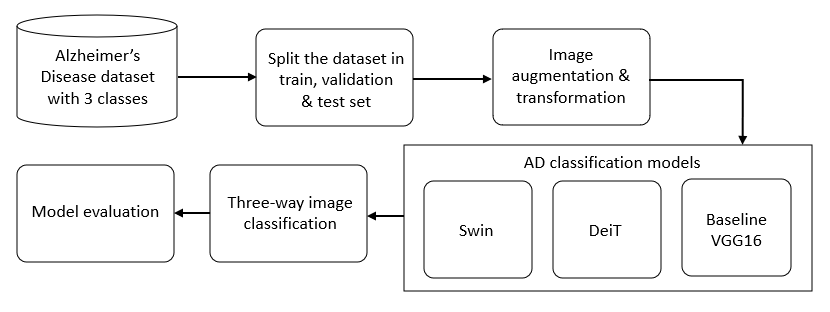
\includegraphics[width=\textwidth]{Methodology flowchart.png}
    \caption{Flowchart summarizing the methodology and experimental setup}
    \label{fig:flowchart}
\end{figure}

\subsection{Hardware and software} \label{subs:ware} 
Training deep learning models requires a large amount of computational power. The local GPU was not sufficient for this research, hence, Google Colab was used. Google Colab is a product from Google Research. It is a hosted Jupyter notebook service that provides access to computing resources such as GPU. The models are trained with Google Colab Pro on a single Tesla T4 GPU with CUDA version 11.2. Training speed was even further increased by storing the dataset in memory. Google Colab provides 12GB of memory, which was sufficient for this research. Python 3.7.15 was the programming language used within Google Colab. The installed packages include Numpy 1.21.6, Scitkit-learn 1.0.2, Matplotlib 3.2.2, Timm 0.6.12, Torch 1.12.1, and Torchvision 0.13.1.

\subsection{Dataset description} \label{subs:dataset} 
The dataset used in this study is a pre-processed dataset available on Kaggle. \citeauthor{Dubey2019AlzheimersImages}, the creator of the dataset, hand-collected the images from various websites with every label verified. It originally had 4 classes: ‘non demented’, ‘very mild demented’, ‘mild demented’, and ‘moderate demented’. Based on ‘The Global Deterioration Scale for Assessment of Primary Degenerative Dementia’ (GDS), non demented can be linked to CN, mild demented to MCI, and moderate demented to AD \citep{Reisberg1982TheDementia}. Demographics of the patients and further information such as if the MRI images are T1 or T2 weighted are unfortunately not included. Results from this study need to be interpreted carefully since the original class descriptions do not match the terminology used in literature and a comprehensive dataset description is lacking. The class ‘very mild demented’ was excluded from the dataset, because it had no clear link in the GDS to the terminology used in other research. After the exclusion of the very mild demented class 4160 jpg images remained in the dataset. The data was split into a training, validation and test set with the splitfolders function. After splitting the data, the training dataset contained 70\% of the images, and the validation and test set each contained 15\% of the images. In the training set, the non demented class contains 2240 images, the mild demented class 627 images, and the moderate demented class 44 images. How this class imbalance is addressed is explained in subsection~\ref{subs:models}


\subsection{Data augmentation and transformation} \label{subs:aug} 
\cite{Touvron2021TrainingAttention} stress the importance of data augmentation for small-scale datasets when working with ViTs. \cite{Ebrahimighahnavieh2020DeepReview}, came to the same conclusion with regard to the CNNs. The DeiT study by \cite{Touvron2021TrainingAttention} found that repeated augmentation \citep{Berman2019MultiGrain:Instances,Hoffer2020AugmentRepetition} was a key factor for successful training, together with RandAugment \citep{Cubuk2020Randaugment:Space}, Mixup \citep{Zhang2018MixUp:Minimization}, Cutmix \citep{Yun2019CutMix:Features}, and Random Erasing \citep{Zhong2020RandomAugmentation}. Due to time restrictions, only Random Erasing was implemented from the DeiT study. Other augmentations are added to make sure that the generalization benefits are not lost. Next to Random Erasing, the augmentations that are added include Horizontal Flip, Vertical Flip, and Color Jitter. The images are resized into shape 256x256 through the transform function from the torchvision library. Subsequently, the images are center cropped to size 224x224, which is the required input size for all the models. After the images are center cropped, they are transformed to a tensor and normalized. In Figure~\ref{fig:sample} sample images are shown with their labels after augmentation and transformation.

\begin{figure}[h]
    \centering
    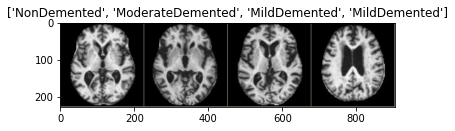
\includegraphics[width=\textwidth]{Sample images.png}
    \caption{Sample images with their label after augmentation and transformation}
    \label{fig:sample}
\end{figure}

\subsection{Models} \label{subs:models} 
All models are pre-trained on ImageNet-1K, which contains 1.33M images from 1000 classes. Having the models pre-trained on the same dataset ensures that model comparison is done on the same grounds. The model layers are frozen so that the knowledge is kept that was gained from pre-training on ImageNet. Only the last two dense layers of the VGG and the last Transformer blocks from the DeiT and Swin are unfrozen so that they are better able to learn the features needed to classify AD. After freezing the model, the classification head is adjusted so that the classification layers can adapt to the given AD classification task. The dataset is heavily imbalanced, which is accounted for by using class weights in the loss function of all the models. The over-sampled non demented class was given a class weight of 1. The mild demented and moderate demented classes are given a class weight of 3.5 and 51 respectively. The class weights are chosen so that when the number of samples in the class would be multiplied by the class weight, the result would be a number close to the number of images in the over-sampled class. All models are run for 50 epochs with a batch size of 32. An extensive description of every model after fine-tuning is given in their respective subsections.


\subsection{VGG16} \label{subs:VGG} 
VGG16 is used as the baseline model in this study because it achieved great performance in prior AD classification literature \citep{Billones2017DemNet:Impairment,Hon2017TowardsLearning,Jain2019ConvolutionalImages}. The model is unique compared to other CNNs because it had a very large amount of 16 convolutional layers with small 3x3 convolution filters \citep{Simonyan2014VeryRecognition}. The study by \cite{Jain2019ConvolutionalImages} achieved the best performance for three-way AD classification. Hence, largely the same architecture and hyperparameters are used for the VGG16 model in this research. \cite{Jain2019ConvolutionalImages} take the pre-trained VGG16 and replace the classification head with a flatten layer, followed by a dense layer with 256 neurons and ReLU activation, a dropout layer with value 0.5, and finally an output layer with 3 neurons. This exact architecture is used in this research. It results in a model with 21M parameters, of which 11M are trainable. The VGG16 model is implemented via the ‘torchvision.models.vgg16’ function. It uses RMSprop as optimizer with a 0.0001 learning rate. The study by \cite{Jain2019ConvolutionalImages} used no learning rate scheduler, whereas our model has a step learning rate scheduler with step size 3 and a gamma of 0.97. Cross-Entropy is used as the loss function, where the class weights discussed earlier are given as parameters. This ensures that the loss function is updated more heavily for under-sampled classes. 

\subsection{DeiT} \label{subs:deitmethod}
Unlike CNNs, the ViT as proposed by \cite{Dosovitskiy2020AnScale} has no convolutional layers. 
The DeiT from \cite{Touvron2021TrainingAttention} builds upon the ViT. It adds a novel distillation procedure by adding a distillation token that interacts with the class token and patch tokens. The class and distillation tokens are learned through back-propagation. Implementation of the distilled version of DeiT was too complicated considering the time constraint for this study. However, they also have a version of the DeiT without the teacher-student mechanism. As discussed in the related work section, data augmentations are another key factor in performing well on small-scale datasets. Hence, the basic DeiT-B is used and several data augmentations are applied. The data augmentations are listed in subsection~\ref{subs:aug}. The DeiT model with pre-trained weights is loaded through the timm library with the timm.create\_model function from \citeauthor{Wightman2022PyTorchModels}. After loading the model, the main architecture is frozen. The classification head is replaced and now consists of a dense layer with 512 neurons and a ReLU activation, which is followed by a dropout layer with value 0.3 and another dense layer with 3 output neurons. The dropout value was set to 0.3 even though the original DeiT does not use a dropout layer. This was done because the excluded data augmentations techniques are good for regularization. Excluding those might lead to overfitting, which is why a dropout layer was added to account for the regularization. The complete DeiT-B model has 86M parameters of which 7.5M are trainable. Again the Cross-Entropy loss function is used, and class weights are added to deal with the class imbalance. Similar to the study by \cite{Touvron2021TrainingAttention}, the AdamW optimizer was chosen with a learning rate of 0.001. AdamW modifies the weight decay in Adam by decoupling weight decay and loss-based gradient updates \citep{Loshchilov2019DecoupledRegularization}. Due to implementation issues, another learning rate scheduler was used. Where \cite{Touvron2021TrainingAttention} used a cosine learning rate scheduler, this study used a step learning rate with a step size of 3 and a gamma of 0.97. 

\subsection{Swin} \label{subs:swinmethod}
\cite{He2022TransformersReview} concluded that one of the main problems of using ViTs in the medial image analysis domain was the need for a large amount of computational power. The computational power needed to calculate the self-attention scales quadratically with respect to image size due to the global self-attention mechanism \citep{Dosovitskiy2020AnScale}. To solve this problem, \cite{Liu2021SwinWindows} created the Swin Transformer. The Swin Transformer calculates the self-attention only within a local window. This window shifts over the image in a non-overlapping manner. The initially small image patches are merged with their neighboring patches for every deeper layer in the model. The Swin Transformer is still able to capture cross-window relationships because of the merging patches. \cite{Liu2021SwinWindows} made the Swin base model (Swin-B) equal in model size to ViT-B and DeiT-B. The Swin Transformer divides the image into patches after which it linearly embeds these patches. The patches are then fed into a Swin Transformer block. This block consists of a multi-head self-attention (MSA) module and a MLP with a GELU activation function in between. A LayerNorm layer is placed before every MSA module and MLP. After each module, a residual connection is applied. The classification head for the DeiT-B was also applied to the Swin-B model. The resulting model has 87M parameters of which 13M are trainable. The hyperparameters in the study by \cite{Liu2021SwinWindows} are largely copied from the DeiT article, and thus we kept the hyperparameters similar to the DeiT. This ensures fair model comparison. The Swin-B model was also implemented through the timm.create\_model function.



\subsection{Evaluation metrics} \label{subs:metrics}
Several evaluation metrics are used to evaluate the performance of the models for the AD multi-class classification task. The evaluation metrics that will be used are accuracy, precision, recall, and the F1-score. Finally, the total training time will be compared to see if the Swin Transformer had any computational benefits, as the study claims. The models are evaluated on the unseen test set, which indicates how well they generalize and how robust the models are. Cross-validation was not performed due to time constraints, however, this would have likely increased the robustness of the models. As discussed in the introduction, classifying MCI correctly is the most important and difficult task. The GDS shows that the mild demented class represents the MCI discussed in literature. Therefore, the main focus will be on the recall of the mild-demented class. All the evaluation metrics are discussed in more detail below. These are derived from the confusion matrix and the classification report that are computed for every model. 


The accuracy is defined as the proportion of the total number of correct predictions. For this multi-class classification problem, this would mean that all the predictions that are correctly classified as non-demented, mild-demented or moderate-demented are added up and divided by the total number of predictions. Accuracy is a widely used metric to evaluate model performance. However, accuracy is a better performance metric when the dataset is balanced. The dataset used has class imbalance which is why we need to look at other performance metrics as well.

Precision indicates the percentage of correct positive predictions relative to the total number of positive predictions. For precision, both the macro-average and precision per class are reported. We look at this metric per class because we have a multi-class classification task. For example, if we want to calculate the precision of the mild demented class, then we need to divide the amount of times that our model correctly classified mild demented by the total amount of times it predicted a case to be mild demented. 

Recall is defined as the proportion of positive cases that are identified correctly. This is calculated by dividing the amount of times a class was correctly predicted as positive by the total number of positive classes. This is the most important metric because it tells how many mild-demented patients are correctly classified. Recall should be as high as possible to maximize the amount of mild-demented patients that can be diagnosed and treated.

The F1-score is calculated by computing the harmonic mean between the precision and recall. Although it is a widely used metric, it should be interpreted with care. The F1-score gives equal weight to precision and recall. For this study, a higher recall is more desirable. This means that a model with the highest F1-score is not necessarily the best model for the given task. 



\newpage


\section{Results}
This section is divided into two parts. Firstly, the overall performance of the models is presented. After that, a subsection will be devoted to the performance of the models with regard to the mild demented class, since this is the most important class for this study. The overall performance will be measured based on accuracy, precision, recall, the F1-score, and training time. Both the DeiT-B and Swin-B model will be compared to the VGG16 baseline model. The performance metrics are measured on the unseen test set to evaluate generalization. In Table~\ref{tab:poverall} the performance metrics are displayed for every model. Table~\ref{tab:pperclass} shows the performance of the models per class.


\begin{table}[b]
    \begin{tabular}{@{}lrrrrl@{}}
        \toprule
        \textbf{Model} & \multicolumn{1}{l}{\textbf{Accuracy}} & \multicolumn{1}{l}{\textbf{Precision}} & \multicolumn{1}{l}{\textbf{Recall}} & \multicolumn{1}{l}{\textbf{F1-score}} & \textbf{Computation time} \\ \midrule
        VGG16          & \textbf{0.9185}                       & \textbf{0.8888}                        & \textbf{0.8942}                     & \textbf{0.8914}                       & \textbf{18 minutes}       \\
        DeiT-B         & 0.8770                                & 0.7688                                 & 0.8720                              & 0.8075                                & 42 minutes                \\
        Swin-B         & 0.8610                                & 0.7078                                 & 0.8005                              & 0.7411                                & 37 minutes                \\ \bottomrule

    \end{tabular}
    \caption{Performance metrics for the VGG16, DeiT-B and Swin-B model. The precision, recall and F1-score are macro averages.}
    \label{tab:poverall}
\end{table}

\subsection{Overall performance} \label{subs:overall}
SQ1 examines how well the DeiT-B model performs compared to the VGG16 baseline model. As can be seen in Table~\ref{tab:poverall} the VGG16 outperformed the DeiT-B model by 4.2\%. The VGG16 and DeiT-B achieved an accuracy of 91.9\% and 87.7\% respectively. SQ2 investigates the Swin-B model compared to the VGG16. The VGG16 beat the Swin-B with an even larger difference of 5.8\%. The Swin-B model achieved an accuracy of 86.1\%. For the precision, recall, and F1-score the macro-averaged values are chosen. The macro-averaged values take the average of all the classes for a given metric. The macro-averaged values are chosen instead of the weighted-average values because the weighted-average values take into account the size of the classes. Using the weighted-average values would make the results appear better than they are because the heavily over-sampled non demented class performed great on all metrics. However, this research focuses on correctly predicting the mild demented class, it would be more appropriate to use the macro-averaged values. For the rest of this subsection, when the precision, recall, or F1-score is mentioned, it means that it is the macro-average of the metric. The VGG16 achieved an 88.9\% precision, beating both the DeiT-B and Swin-B with a precision of 76.9\% and 70.1\% respectively. This means that the VGG16 model had the highest percentage of actually positive instances out of the predicted positive instances. The recall of the DeiT-B is 87.2\%, which is 2.2\% lower than the recall of 89.4\% for the VGG16 model. The recall gap between the VGG16 and Swin-B is a lot bigger, namely 9.3\%. The Swin-B model achieved a recall of 80.1\%. This shows that the Swin-B overall is the worst at correctly identifying all the classes, whereas the VGG16 model performs the best. For the F1-score the differences between the models become quite substantial. The VGG16 model achieved an F1-score of 89.1\%, whereas the DeiT-B and Swin-B achieved an F1-score of 80.8\% and 74.1\% respectively. This difference can be explained by the fact that the F1-score gives an overall score of the precision and recall together, however, it weighs lower scores heavier. The precision and recall for the VGG16 are almost similar. However, for the DeiT-B and Swin-B model, there is a larger difference between the precision and recall, which weighs the harmonic mean of the two metrics down. The VGG16 model was 24 minutes faster in training than the DeiT-B model, and 19 minutes faster than the Swin-B model. The VGG16 model completed training in 18 minutes, the DeiT-B in 42 minutes, and the Swin-B in 37 minutes. It was expected that the ViTs would take longer because the attention needs to be computed. That Swin-B is faster than the DeiT-B can be explained by the fact that the Swin-B has linear computational complexity with respect to image size instead of the quadratic computational complexity of the DeiT-B.


\subsection{Performance on the mild demented class} \label{subs:mild}
To treat or mitigate any of the negative developments a patient might experience due to AD, it is of vital importance to detect the prodromal stage of AD as early as possible. Therefore this section will specifically look at the performance of the models with regard to the mild demented class. The precision of the DeiT-B model for the mild demented class is 73.8\%. This indicates that when the DeiT-B model predicted an instance to be mild demented, it was right 73.8\% of the time. The VGG16 outperformed the DeiT-B here by 6.8\%, as the VGG16 achieved a precision for the mild demented class of 80.6\%. The Swin-B model was also beaten by the VGG16. It achieved a precision of 70.9\% for the mild demented class which is considerably lower than the VGG16. Although having a low precision is not desired, it does not mean that a model is worse. Especially when taking into account the goals of this research. Generally, there is a trade-off between precision and recall. Recall for the mild demented class might be the most important metric for this research, as it describes what percentage of people that belong to the mild demented class are correctly classified. This is where the VGG16 model really comes out on top over the ViTs. The VGG16 model achieved a recall of 83\% on the mild demented class. Indicating that it would correctly classify 83\% of the patients that are mild demented. The DeiT-B scored a substantial 14.1\% lower than the VGG16, with a recall of 68.9\%. Swin-B performs even worse than the DeiT-B, having a gap of 16.3\% compared to the baseline model. Swin-B correctly classifies 66.7\% of the mild demented patients. In Table~\ref{tab:pperclass} it can be seen that all models score the lowest recall for the mild demented class. 

In conclusion, when looking at the accuracies of the models, it is clear that the VGG16 has the advantage over the DeiT-B and Swin-B in this setup. Looking at the recall scores on the mild demented class further confirms this finding. 


\begin{table}[]
    \centering
    \begin{tabular}{@{}llrrr@{}}
    \toprule
    Model & Class & \multicolumn{1}{l}{Precision} & \multicolumn{1}{l}{Recall} & \multicolumn{1}{l}{F1-score} \\ \midrule
             & VGG16  & \textbf{0.9517} & \textbf{0.9437} & \textbf{0.9477} \\
    Non      & DeiT-B & 0.9213          & 0.9271          & 0.9242          \\
             & Swin-B & 0.9148          & 0.9167          & 0.9157          \\ \midrule
             & VGG16  & \textbf{0.8058} & \textbf{0.8296} & \textbf{0.8175} \\
    Mild     & DeiT-B & 0.7381          & 0.6889          & 0.7126          \\
             & Swin-B & 0.7087          & 0.6889          & 0.6870          \\ \midrule
             & VGG16  & \textbf{0.9091} & 0.9091          & \textbf{0.9091} \\
    Moderate & DeiT-B & 0.6471          & \textbf{1.000}  & 0.7857          \\
             & Swin-B & 0.5000          & 0.8182          & 0.6207          \\ \bottomrule
    
    \end{tabular}
    \caption{Performance metrics for the VGG16, DeiT-B and Swin-B model. The precision, recall and F1-score are macro averages.}
    \label{tab:pperclass}
\end{table}

\newpage

\section{Discussion}
A recent study by \cite{Turknett2022DemandDementia} concluded that a growing number of studies find that lifestyle and environment could be key predictors of AD development \citep{Yu2020Evidence-basedTrials.,Sundstrom2020ARisk}. Specifically, a decline in cognitive demand over the lifespan was indicated as the main driver of AD progression \citep{Turknett2022DemandDementia}. Because of these findings, non demented and mild demented patients now have more concrete practical implications to battle the disease. Especially for mild demented patients it is important because the complete conversion to AD could be prevented by incorporating cognitively harder tasks in their day-to-day life. This could mitigate the negative AD trends mentioned in the introduction. Therefore, improving the performance of deep learning models in this field is vital. The relatively new ViTs and their variations have achieved promising results in prior research \citep{Fang2021YouDetection, Ye2019Cross-modalSegmentation, Dosovitskiy2020AnScale}. However, the investigation of their performance for AD classification remains limited, which leads us to the main research question of this study:

\begin{quote}
\centering
\emph{How do Vision Transformers perform in classifying multiple Alzheimer’s Disease stages?}
\end{quote}

A literature review by \cite{He2022TransformersReview} showed that two main problems arise when applying ViTs to medical image classification, namely a lack of large-scale datasets and high computational needs. The following sub-questions are formulated based on these problems:

\begin{itemize}
\centering
    \item[SQ1] \emph{How does the data-efficient Vision Transformer compare to the baseline 2D CNN in classifying multiple AD stages?}
    \item[SQ2] \emph{How does the computationally-efficient Vision Transformer compare to the baseline 2D CNN in classifying multiple AD stages?}
\end{itemize}

\cite{Touvron2021TrainingAttention} developed the DeiT model, largely based on the standard ViT from \cite{Dosovitskiy2020AnScale}. The DeiT model should be able to handle small-scale datasets better. The hierarchical Swin Transformer by \cite{Liu2021SwinWindows} should resolve the problem of high computational needs because of its linear computational complexity compared to the quadratic computational complexity of other ViT models. Therefore, to resolve the issues mentioned by \cite{He2022TransformersReview}, the DeiT-B and Swin-B model are proposed for this research. Some studies conclude that ViTs are slowly beating the state-of-the-art CNNs \citep{Matsoukas2021IsImages}, which is why the DeiT-B and Swin-B models are compared to the VGG16. In this research, the VGG16 model uses a similar architecture as in the study by \cite{Jain2019ConvolutionalImages}. They achieved state-of-the-art performance on three-way AD classification. 

\subsection{Sub-question 1} \label{subs:sq1}
To answer SQ1, the results of the DeiT-B are compared to the baseline VGG16 model. With a 4.2\% difference, the VGG16 model beat the DeiT-B based on accuracy. The main reason for the gap could be explained by the fact that the distilled DeiT version could not be used in this study due to time constraints. \cite{Touvron2021TrainingAttention} show that the novel distillation technique was one of the key factors in the success of their data-efficient ViT. The superiority of the VGG16 model becomes even more clear when the models are compared based on the recall of the mild demented class. Here, the VGG16 outperformed the DeiT-B by a substantial margin of 14.1\%. This large discrepancy was not expected. However, it might be explained by the fact that the MRI scans from patients in the mild demented class might have subtle features that the DeiT-B was not able to detect. The CNN excels at extracting local features \citep{Ebrahimighahnavieh2020DeepReview}, which might explain the difference from the DeiT model. The fact that the VGG16 outperformed the DeiT-B model is in line with \cite{Yin2022SMIL-DeiT:MultipleClassification}. They found that the DeiT-S model was only able to beat the CNN baseline model when using a self-supervision technique for training. When they were not using the self-supervision technique, even the distilled DeiT was not able to outperform the CNN. \cite{Touvron2021TrainingAttention} mention that the hyperparameters used in their study might be sub-optimal, which might be another explanation for the difference between the models. CNN models have been improving ever since their success was widely recognized after the ImageNet LSVRC-2010 competition. It might be too optimistic to expect that ViTs are already able to consistently outperform CNNs. Especially when considering the substantially longer period of continuous improvement for the CNNs. However, the potential for the DeiT is there. Using the distilled version of the DeiT could be a key aspect in bridging the gap to the VGG16 model. 

\subsection{Sub-question 2} \label{subs:sq2}
SQ2 will be answered by comparing the hierarchical Swin Transformer \cite{Liu2021SwinWindows} to the baseline VGG16 model. For medical image classification the computational efficiency of the Swin Transformer can be seen as the main benefit. However, when comparing the VGG16 and Swin-B model, it shows that the Swin-B model takes twice as long to train compared to the VGG16 model. This can be explained by the fact that the Swin-B has to calculate the attention within its local windows. When compared to the DeiT-B, The Swin-B was almost 12\% faster in training. This was expected because the Swin-B has a linear computational complexity compared to the quadratic computational complexity of the DeiT-B. The VGG16 model also outperforms the Swin-B model on all metrics. The large difference in recall for the mild demented class and accuracy raises the question as to why this might be the case. A cause could be that the performance of the Swin-B model might be more heavily impacted than the CNN because of the small-scale dataset. In addition, similar to the DeiT-B, the VGG16 was improved and fine-tuned for a considerably longer time than the Swin. Concluding SQ2, it can be stated that the Swin Transformer did not bridge the gap to the VGG16 in terms of training time as much as hoped. The performance of the Swin-B model was also worse on all metrics. Hence, the Swin-B is not yet able to compete with the VGG16 baseline model in the AD classification domain. At least not in the setting investigated in this study.

\subsection{Limitations} \label{subs:limit}
In this study some useful insights are gained for using ViTs in the AD classification domain. However, this research also has a few limitations. Initially the ADNI dataset would be used for this study. It is the most popular AD dataset used in literature because it is one of the largest, most qualitative, longitudinal AD datasets that exist up to date \citep{Ebrahimighahnavieh2020DeepReview}. Unfortunately the dataset had to be discarded due to some pre-processing issues with the 3D MRI data. This meant that an already pre-processed dataset from the Kaggle website had to be used. The limitation of this dataset is that it lacked information on subjects and the dataset itself. The dataset description only mentioned that the dataset was hand collected from various websites and that the labels were verified. Moreover, it is expected that the models do not generalize well on slices from different planes or on images that are pre-processed differently. Due to time constraints it was not possible to perform k-fold cross-validation, which would have improved the robustness of the models. Another limitation is that the class descriptions of the dataset from the Kaggle website do not exactly match the terminology used in literature. By using the GDS from \cite{Reisberg1982TheDementia}, the relation to the literature can be made with some caution. However, it would be better to use a dataset that uses class descriptions similar to the ones in literature. Another limitation is that for the DeiT model not the same exact data augmentations were performed and that the distilled version of the DeiT model was not implemented. The novel distillation technique reportedly was one of the main factors for the success of the DeiT on small-scale datasets. Thus, conclusions about the performance of the DeiT-B model need to be interpreted carefully. Model performance would likely have improved when the same data augmentations and the distilled version would have been implemented. Lastly, research has shown that using multiple modalities and biomarkers remains the preferred method for AD classification. In this research only the slice-based method was used due to the heavily increased complexity when combining modalities or biomarkers.

\subsection{Recommendations for future research} \label{subs:future}
For future research it is recommended to work with datasets from verified sources like ADNI. They have experts that are able to correctly label the data in conjunction with other metrics such as the MMSE score and the LM test. Although the ADNI dataset provides high-quality MRI data, it is still a relatively small dataset. Hence, we emphasize the need for a large-scale AD dataset, on which the ViTs should be able to perform better. To increase the dataset quality and size, it is recommended to take multiple slices from a single patient that are selected based on entropy. This will ensure that only the most relevant slices are used. In addition, the performance from the DeiT-B model might be lower due to not being able to implement the optimal training procedures as described in the study by \cite{Touvron2021TrainingAttention}. Using the distilled DeiT version and the same data augmentations as in the study will likely improve the performance of the DeiT model. Finally, further investigation is needed for different fine-tuning and architectural choices for both the DeiT and Swin. Since these ViT models have only been published relatively recently, further improvements can probably be made for AD classification by testing different training procedures and hyperparameters. 

\newpage

\section{Conclusion}
This study investigated the performance of ViT models on three-way AD classification. As the number of AD patients, deaths caused by AD, and healthcare costs for treating AD are all increasing, improving the methods for early detection of the disease becomes crucial. Detecting mild demented patients early might provide for opportunities to slow down or completely prevent the conversion to AD. The insights from the study by \cite{Turknett2022DemandDementia} may provide for more concrete intervention points for mildly demented patients, namely the incorporation of cognitively harder tasks in their day-to-day life. The DeiT and Swin models are compared to the state-of-the-art 2D CNN as a baseline. The VGG16 was taken as the baseline model, largely having the same architecture as a study by \cite{Jain2019ConvolutionalImages}, which achieved great performance on three-way AD classification. Both the DeiT-B and Swin-B model are outclassed on all performance metrics by the 2D CNN. However, the DeiT study by \cite{Touvron2021TrainingAttention} points out that CNNs have been under development for multiple years, whereas their DeiT needs more research to find the optimal set of hyperparameters. Especially the DeiT-B model has some great potential. It performed reasonably even though not all training procedures from the original DeiT study by \cite{Touvron2021TrainingAttention} could be implemented. The Swin-B did train faster than the DeiT. However, this did not make a noteworthy difference, because training time was not an issue for this study. It can be concluded that although the 2D CNN still reigns supreme in the AD classification domain, there might be some great potential for ViTs and especially the DeiT model once the training procedures, fine-tuning and hyperparameters are all optimized.

\newpage

\bibliography{references}


\end{document}